\documentclass{beamer}
\usepackage{hyperref}
\usepackage{xcolor}
\usepackage{graphicx}
% Theme choice:
\usetheme{CambridgeUS}

% Title page details: 
\title{Modelo predictivo del crecimiento poblacional} 
\subtitle{Equipo \#2}
\author{\textit{Estimación de la capacidad de carga }}
\date{\today}
\logo{\large \LaTeX{}}

\begin{document}

% Title page frame

\begin{frame}
    \titlepage 
    \underline{\textbf{Integrantes: }}\\
    Guillermo Cepero García \\ Luis Ernesto Serras Rimada \\ Miguel Vadim Vilariño Pedraza
\end{frame}

% Remove logo from the next slides
\logo{}
\author{\textit{\underline{\textbf{Equipo \#2}}}}

\section{Introducción}
\begin{frame}{Modelo de crecimiento poblacional}
    El análisis del crecimiento poblacional reviste gran importancia debido a su relevancia en diversos campos como la economía, demografía, epidemiología y la ecología. Resulta útil en múltiples ámbitos, incluyendo estudios demográficos, planificación urbana y análisis de recursos naturales.
\end{frame}

\begin{frame}{Objetivos}
    Objetivos principales:\\
\begin{itemize}
    \item Estimar el numero maximo de personas que
        pueden ser sostenidamente alojadas en un area
        geografica determinada y evaluar el equilibrio entre la poblacion existente y la capacidad de carga
        ambiental
    \item Contribuir al diseno de estrategias de planifi-
        cacion urbana y rural que equilibren el crecimiento
        economico con la proteccion del medio ambiente y
        los servicios basicos.
    \item Permitir evaluar el impacto potencial del cambio
        climatico y otros factores externos en la capacidad
        de carga poblacional a largo plazo.
    \item Contribuir al diseno de programas de educacion
        ambiental y concientizacion sobre las implica-
        ciones del crecimiento poblacional.
    \item Ayudar a establecer limites razonables para el
        crecimiento demografico, evitando excederse en
        la explotacion de recursos naturales y servicios
        puublicos.
\end{itemize}

\end{frame} 

\section{Ecuación Diferencial}
\begin{frame}{Modelo logístico}
    Se plantea trabajar el asunto con un modelo matemático que nos pueda conducir a dicha prediccion, y se considera 
    el \textbf{modelo del crecimiento logístico}, que es solución de la ecuación diferencial que describe cómo la tasa de crecimiento de la población (dP/dt) 
    cambia con el tamaño de la población (P(t)) $$\frac{dP}{dt} = r \cdot P(t)(1 - \frac{P(t)}{K}) $$
\end{frame}
\begin{frame}
donde se tiene que:
\begin{itemize}
    \item (P(t)) es la población en función del tiempo (t).
    \item (r) es la tasa de crecimiento intrínseca de la población.
    \item (K) es la capacidad de carga o tamaño máximo sostenible de la población.
\end{itemize}\\

\textit{\underline{Parámetros a Estimar:}}
\begin{itemize}
    \item (r): Tasa de crecimiento intrínseca de la población. 
    \item (K): Capacidad de carga de la población.
\end{itemize}
\end{frame}

\section{Modelo Matemático}
\begin{frame}{Modelo del crecimiento logístico}
    \underline{La ecuación del modelo logístico del crecimiento poblacional tiene la forma:} $$P(t) = \frac{K}{1 + Ae^{-rt}}$$
    \underline{La ecuación para encontrar (A) es:} $$P(0) = \frac{K}{1 + Ae^{0}}$$
\end{frame}

\begin{frame}
    (A) es una constante que depende de las condiciones iniciales de la población. Esta función muestra claramente 
    el punto de inflexión, donde la tasa de crecimiento cambia de positiva a negativa, indicando que la población 
    ha alcanzado su capacidad de carga y está comenzando a estabilizarse.
\begin{center}
    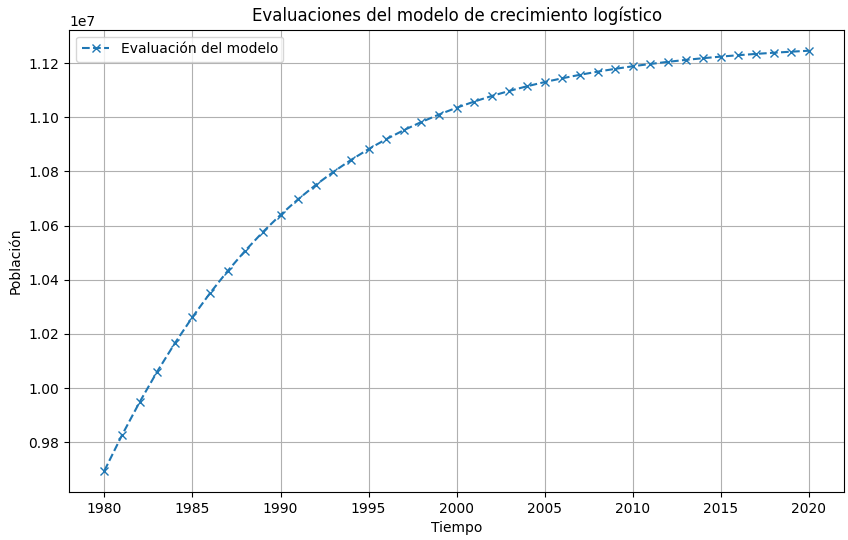
\includegraphics[width=0.45\textwidth]{img/model.png}$^{5}$\\
\end{center}
\end{frame}

\section{Implementación en Python}
\begin{frame}{curvefit}
    Se utilizaron los datos históricos de densidad poblacional desde 1980 hasta 2020 publicados en las series estadisticas del sitio web de la ONEI. Y se desean ajustar los parámetros de la capacidad de carga($K$) y la tasa ($r$).
    Para ello se decide utilizar la aproximación por mínimos cuadrados por medio de la función curvefit del módulo scipy.optimize en Python, cuya función matemáticamente se puede representar como:\\
    Minimizar: $\sum_{i=1}^{N} (y_{i} - f(x_{i}, \theta))^2 $ \\
\end{frame}

\begin{frame}{curve-fit}
    Toma los parámetros:
    \begin{itemize}
        \item f: es la función modelo para la optimización.
        \item xdata: son los valores independientes (el tiempo ($t$ como $x_{i}$)).
        \item ydata: son los valores dependientes (los valores de densidad poblacional en función del tiempo ($P$ como $y_{i}$)).
        \item p0: Estimación inicial.
    \end{itemize}
\end{frame}

\begin{frame}
    \begin{block}{\textcolor{red}{Y procede de la forma:}}
    $$min[\sum_{i=1}^{N} (P - (\frac{K}{(P(0)-1)}̇e^{-rt}))^{2}]^{\frac{1}{2}}$$
    \end{block}
La función curvefit intentará minimizar la suma de los cuadrados de los residuales para encontrar los valores óptimos de $K$ y $r$ que minimizan esta expresión. 
\end{frame}

\section{Resultados}
\begin{frame}{Preview de los datos utilizados}
    \begin{center}
        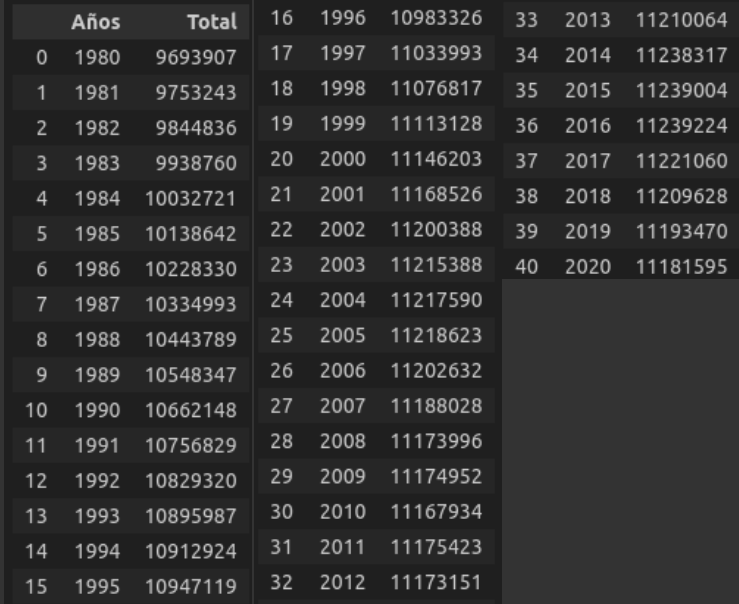
\includegraphics[height = 7cm]{img/data.png}
    \end{center}
\end{frame}
\begin{frame}{Modelo sin intervalos}
    \begin{center}
    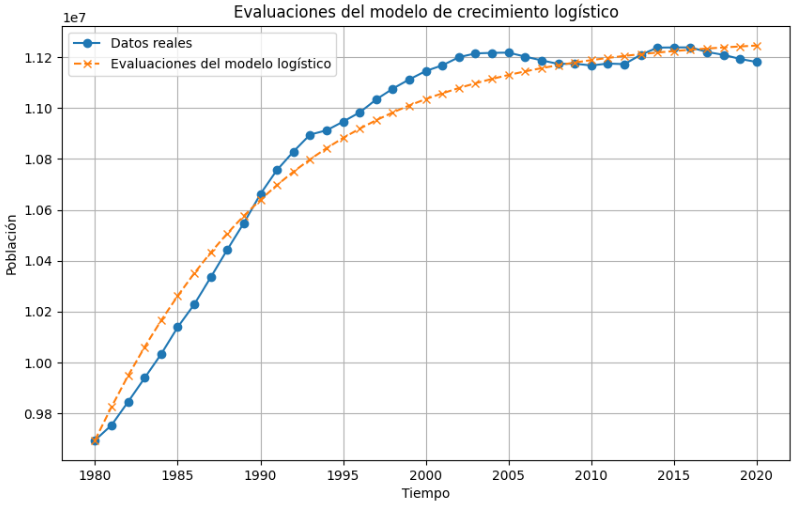
\includegraphics[height = 7cm]{img/real_vs_pred.png}
    \end{center}
\end{frame}

\begin{frame}{Predicción del modelo sin intervalos}
    \begin{center}
        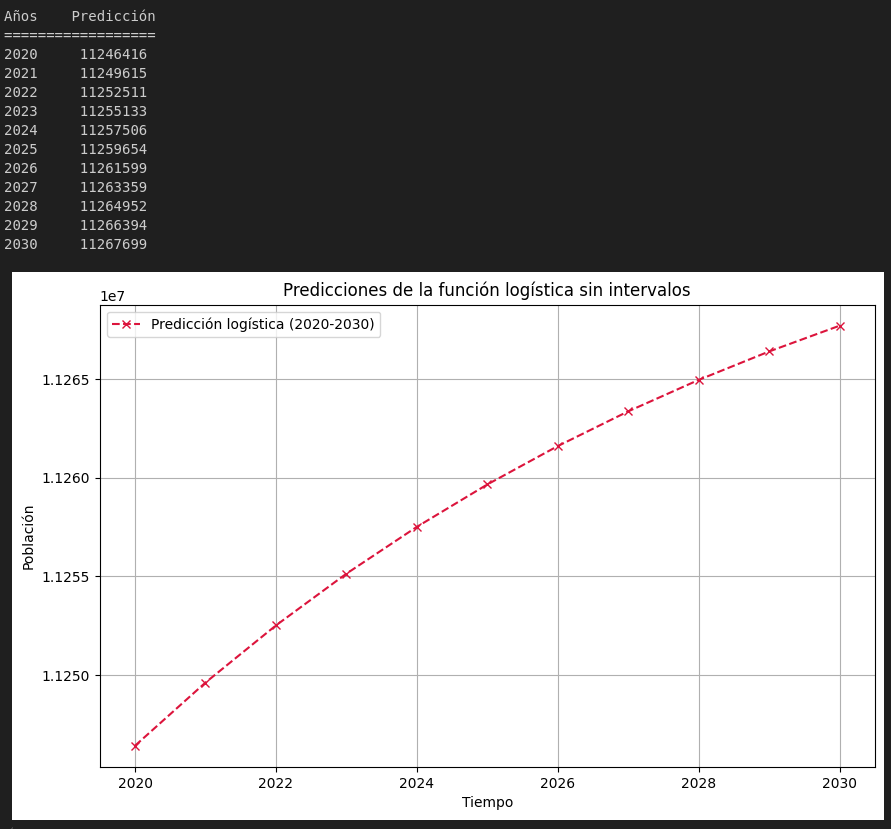
\includegraphics[height = 7cm]{img/graph_sin_intervalos.png}
    \end{center}
\end{frame}

\begin{frame}{DataFrame para intervalos de 5 años}
    \begin{center}
    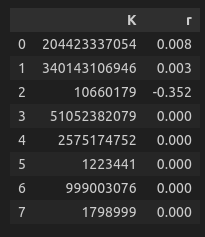
\includegraphics[height = 7cm]{img/df5.png}
    \end{center}
\end{frame} 


\begin{frame}{Predicción para intervalos de 5 años}
    \begin{center}
    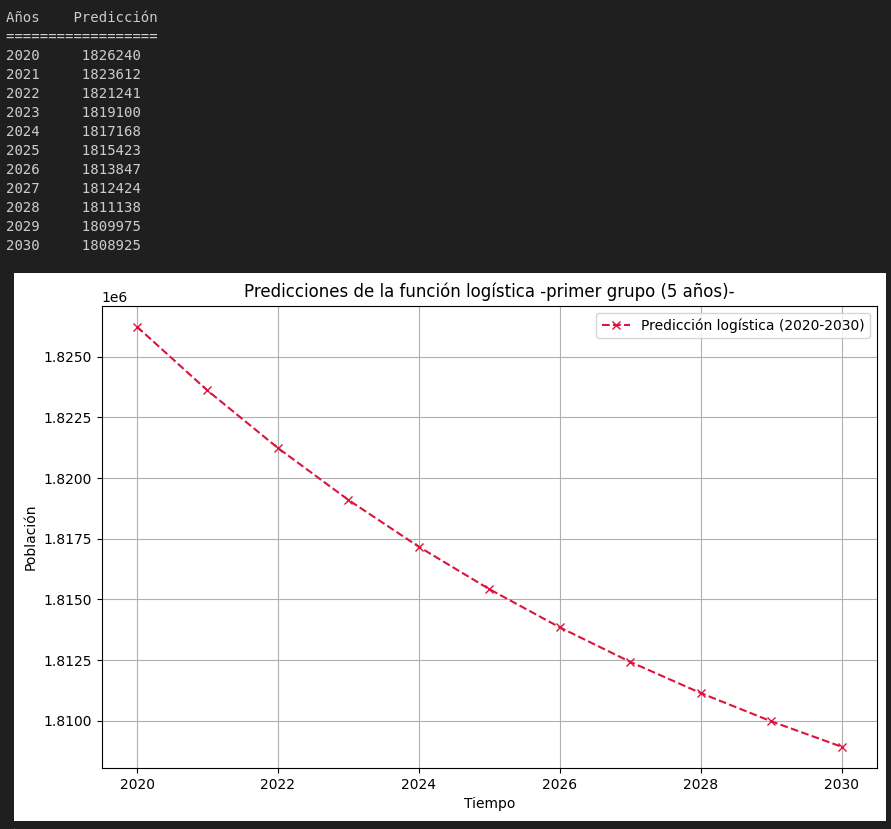
\includegraphics[height = 7cm]{img/df5_graph.png}
    \end{center}
\end{frame}


\begin{frame}{DataFrame para intervalos de 8 años}
    \begin{center}
    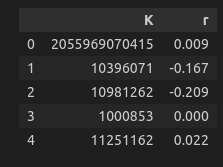
\includegraphics[height = 7cm]{img/df8.png}
    \end{center}
\end{frame} 

\begin{frame}{Predicción para intervalos de 8 años}
    \begin{center}
    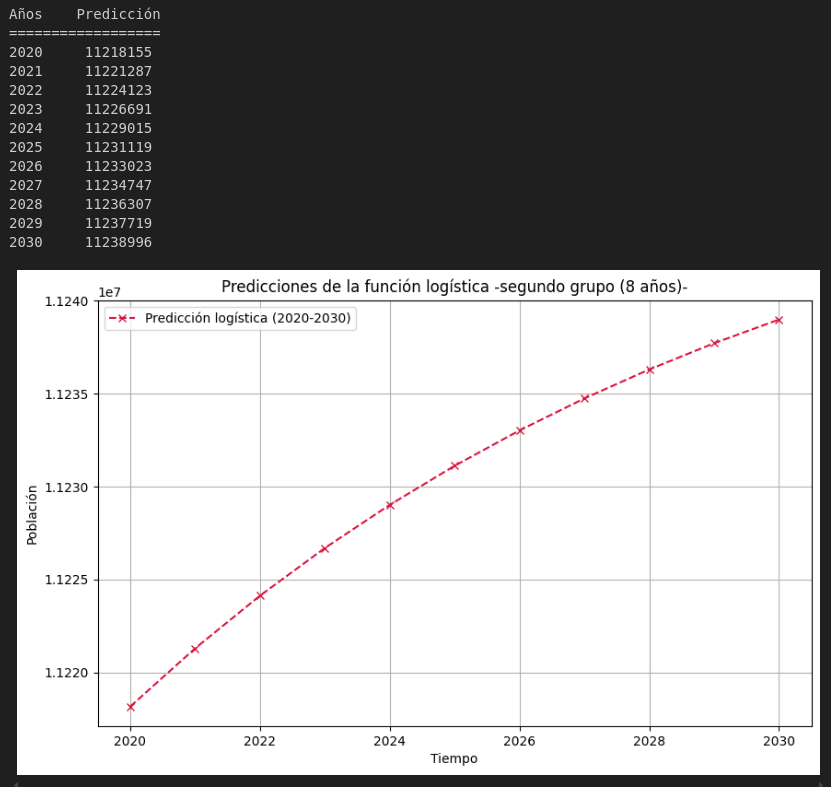
\includegraphics[height = 7cm]{img/df8_graph.png}
    \end{center}
\end{frame}

\begin{frame}{DataFrame para intervalos de 10 años}
    \begin{center}
    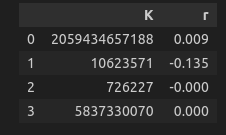
\includegraphics[height = 7cm]{img/df10.png}
    \end{center}
\end{frame} 

\begin{frame}{Predicción para intervalos de 10 años}
    \begin{center}
    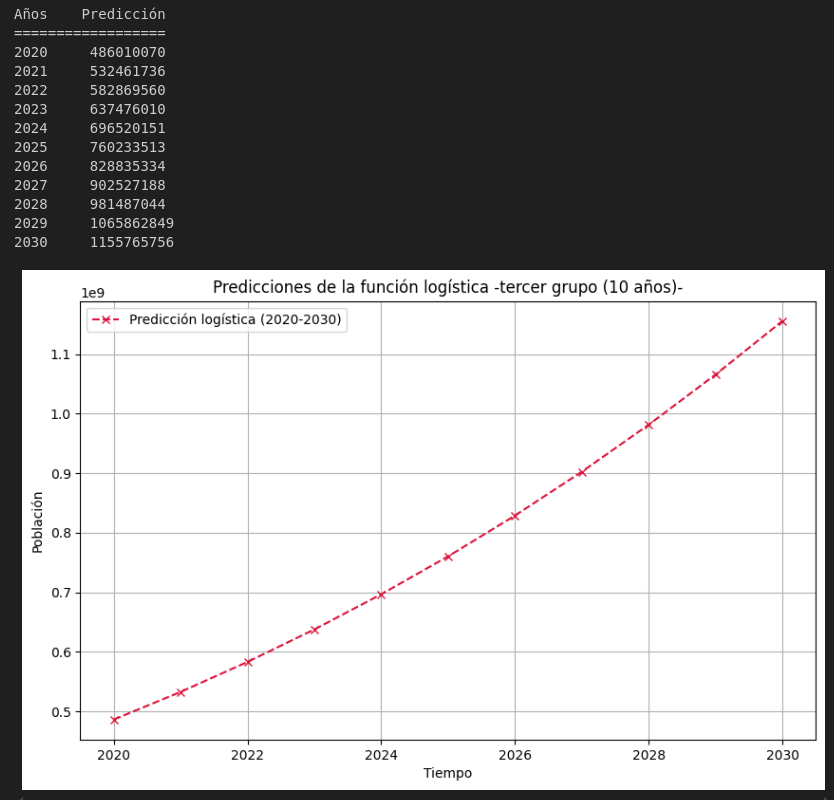
\includegraphics[height = 7cm]{img/df10_graph.png}
    \end{center}
\end{frame}

\section{End}
\begin{frame}{Recomendaciones}
\begin{itemize}
    \item Mejorar el Modelo Matemático
    \item Ampliar la Base de Datos:
    \item Validar y Refinar el Modelo
    \item Investigar Factores Externos
    \item Divulgar los Resultados
    \end{itemize}
    Estas recomendaciones buscan fortalecer el modelo actual, ampliar su alcance y utilidad, y contribuir al conocimiento demográfico de Cuba, teniendo en cuenta las particularidades observadas en el análisis inicial.
\end{frame}

\begin{frame}{Muchas gracias :)}
    \begin{center}
    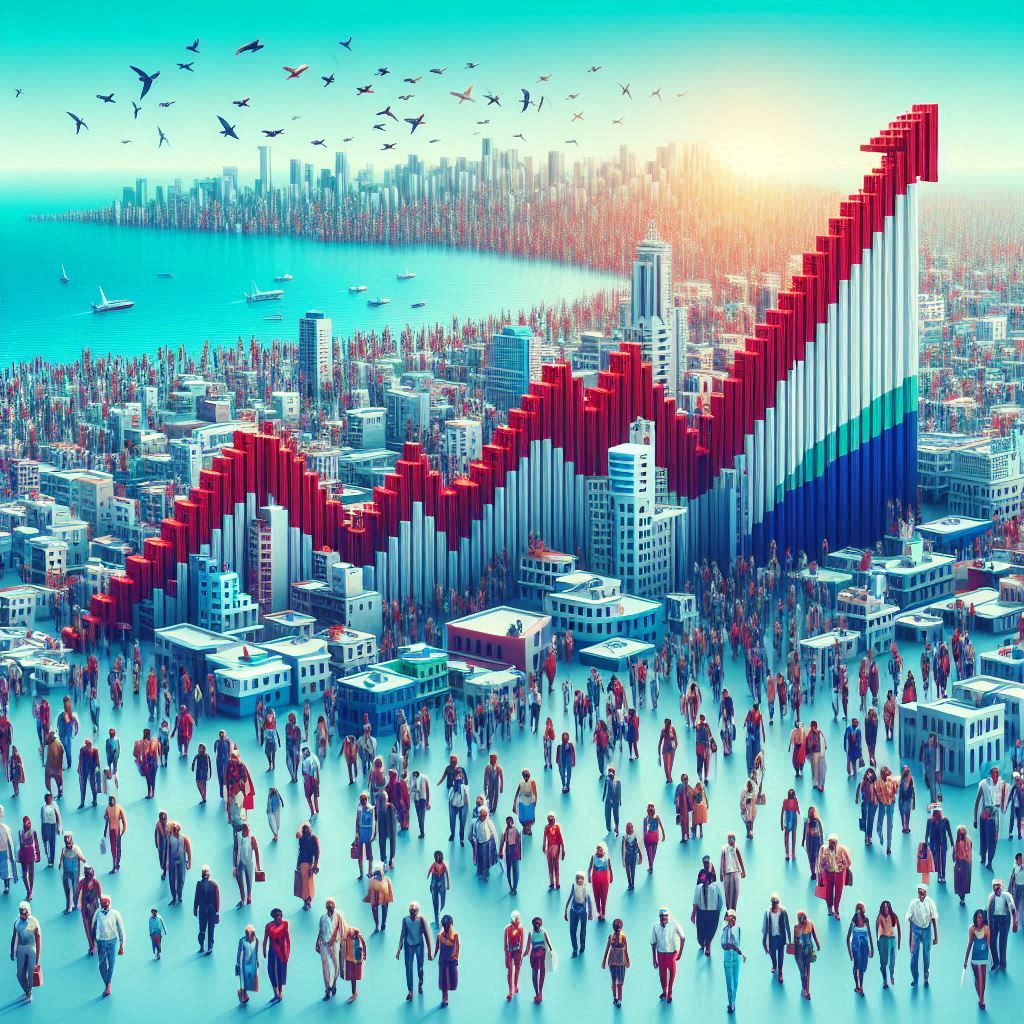
\includegraphics[height = 8cm]{img/cuba1.jpeg}
    \end{center}
\end{frame}

\end{document}